\chapter{Homogeneous Electron Gas}

\section{Exchange and Correlation}\label{s5.1}
The homogeneous electron gas is describe by the Hamiltonian
\begin{eqnarray}
    H &=& \sum_{\bp\sigma} \varepsilon_\bp C^\dagger_{\bp\sigma} C_{\bp\sigma} + \frac{1}{2V} \sum_{\bk\bk'\sigma\sigma'} \sum_{\bq\neq 0} v_q C^\dagger_{\bk+\bq \sigma} C^\dagger_{\bk'-\bq \sigma'} C_{\bk'\sigma'} C_{\bk\sigma} \label{5.1} \\
\varepsilon_p &=& \frac{p^2}{2m} \nonumber \\
v_q &=& \frac{4\pi e^2}{q^2} \label{5.2}
\end{eqnarray}
which was derived in \eqref{1.164}.
The free electrons mutually interact by Coulomb's law.
This $N_e$ electrons in a volume $V$ with the average density $n_0 = \frac{N_e}{V}$.
A positive charge of density $n_0$ is spread uniformly through the volume make the system charge neutrality.
The homogeneous electron gas is also called the \textbf{jellium model} of a solid.

The parameter $r_s$ is universally used to describe the density of an electro gas,
\begin{equation}
    \frac{4\pi n_0 a_0^3}{3} r_s^3 =1 \label{5.3}
\end{equation}
where $a_0$ is the Bohr radius.
$r_s$ is small for high-density electron gas and it is large for a low-density gas.
The density may related to the Fermi vector,
\begin{equation}
    n_0 = 2 \int \frac{d^3 p}{(2\pi)^3} \eta_p = \frac{1}{\pi^2} \int_0^{k_F} p^2 dp = \frac{k_F^3}{3\pi^2}     \label{5.4}
\end{equation}
so the Fermi wave vector and energy are related to $r_s$,
\begin{eqnarray}
    k_F a_0 &=& \frac{1.9192}{r_s} \nonumber \\
    E_F &=& \frac{3.6832}{r_s^2}  E_{ry}, ~ ~ ~ E_{ry}=13.60 eV \label{5.5}
\end{eqnarray}
The plasma frequency is
\begin{equation}
    \hbar \omega_p = \hbar \sqrt{ \frac{4\pi e^2 n_0}{m}  }     \label{5.6}
\end{equation}
In homogeneous electron gas, the average kinetic energy of the electrons is going to be proportional to $\langle E_F \rangle \sim k_F^2$.
Which by dimension analysis, we have $\langle E_F \rangle\propto 1/r_s^2$.
For the Coulomb energy $\langle v_p \rangle \propto 1/r_s$.
When the electron gas is sufficiently hight, $r_s$ is small, the kinetic energy term will be larger than the potential energy term, which means electrons behaves like the free particles.

\subsection{Kinetic energy}
The first energy term is kinetic energy.
The contribution to the ground state energy is obtained by summing over all particles in the ground state
\begin{eqnarray}
    E &=& \sum_{\bp \sigma} \varepsilon_p n_p = 2 V \int \frac{d^3 p}{(2\pi)^3} \frac{p^2}{2m} \eta_p = \left( \frac{N_e}{n_0} \right) \frac{1}{2\pi^2 m} \int_0^{k_F} p^4 dp \nonumber \\
&=& \frac{3}{5} \frac{\hbar^2 k_F^2}{2m} N_e = \frac{3}{5} E_F N_e = \frac{2.2099}{r_s^2} E_{ry} N_e    \label{5.8}
\end{eqnarray}
The average kinetic energy is $ \frac{3}{5} E_F$, which is given in terms of $r_s$.

\subsection{Hartee}
All the remaining terms in the energy come from the Coulomb interaction between the particles.
\textit{The first term which occurs is the Coulomb interaction between the electrons and the uniform positive background}, which is called the \textbf{Hartee interaction}.
In the model of the homogeneous electron gas, the time-averaged electron density is uniform throughout the system, as is the positive background.
These equal and opposite charge cancel each other, and Hartree energy is zero.
The energy is
\begin{equation}
    N_e E_0 = \frac{e^2}{2} \int \frac{d^3 r_1 d^3 r_2}{\abs{\br_1 - \br_2}} \left[ \rho_e(\br_1) - \rho_i(\br_1) \right] \left[ \rho_e(\br_2) - \rho_i(\br_2) \right]  \label{5.9}
\end{equation}
but the ion and electron are $\rho_e = \rho_i = n_0$, then the contribution is zero.
This fact has already been used in \eqref{5.1} by omission of the $\bq=0$ term from the Coulomb interaction.
The $\bq=0$ term is the direct Coulomb interaction among the electrons, and it is omitted because it is canceled by the direct interaction with the positive background.

\subsection{Exchange}
The Coulomb interaction in \eqref{5.1} provide other energy contributions in addition to the direct term.
For Hartee term the corresponding $H$ is given
\begin{equation}
    \sum_{\bk \bk' \sigma \sigma'} \langle C^\dagger_{\bk+\bq,\sigma} C^\dagger_{\bk'-\bq,\sigma'} C_{\bk',\sigma'} C_{\bk,\sigma} \rangle \approx \delta_{\bq = 0} \sum_{\bk\sigma} \langle C^\dagger_{\bk,\sigma} C_{\bk,\sigma} \rangle \sum_{\bk'\sigma'} \langle C^\dagger_{\bk',\sigma'} C_{\bk',\sigma'} \rangle
\end{equation}
Another way to pair the same operator gives
\begin{equation}
    \approx - \sum_{\bk\bk'\sigma\sigma'} \langle C^\dagger_{\bk+\bq,\sigma} C_{\bk',\sigma'} \rangle \langle C^\dagger_{\bk'-\bq,\sigma'} C_{\bk,\sigma'} \rangle = - \sum_{\bk\sigma} n_{\bk+\bq} n_\bk
\end{equation}
This require that $\sigma' =\sigma$ and $\bk' = \bk + \bq$.
This term is called \textbf{exchange energy (Fock energy)}.
\textit{Retaining both terms is called Hartree-Fock.}
The exchange term was derived in \eqref{2.138}, it gives a contribution to the energy of an individual electron, as well as a contribution to the ground state energy of the collection of electrons. \textbf{For per electron},
\begin{equation}
    \Sigma_x(k) = - \frac{1}{V} \sum_\bq v_q n_{\bk+\bq}    \label{5.11}
\end{equation}
\begin{equation}
    E_{gx} = - \sum_{\bk\bq\sigma} \frac{v_q}{2V}   n_{\bk+\bq} n_\bk =\frac{1}{2N_e} \sum_{\bk\sigma} n_\bk \Sigma_x(k)  \label{5.12}
\end{equation}
The self-energy $\Sigma_x(k)$ depends only on the magnitude of the wave vector $k$ of the particle and gives
\begin{eqnarray}
    \Sigma_x(k) &=& - \int \frac{d^3 p}{(2\pi)^3} \frac{4\pi e^2}{\abs{\bp -\bk}^2} n_p \nonumber \\
    &=& - \frac{e^2}{\pi}  \int_0^{k_F} p^2 dp \int_{-1}^{1} \frac{d \cos\theta}{k^2+p^2 -2pk\cos\theta} \nonumber \\
    &=& - \frac{e^2 k_F}{\pi}  \left( 1+ \frac{1-y^2}{2y} \ln \abs{\frac{1+y}{1-y}}  \right) \label{5.16} \\
    y &=& \frac{k}{k_F} \label{5.17}
\end{eqnarray}

A particle at the Fermi energy $k=k_F$ has
\begin{equation}
    \Sigma_x (k_F) = - \frac{e^2 k_F}{\pi} \label{5.18}
\end{equation}
It is convenient to write
\begin{eqnarray}
    \Sigma_x(k) &=& \frac{e^2 k_F}{\pi} S(y)    \label{5.19} \\
    S(y) &=& - \left( 1+ \frac{1-y^2}{2y} \ln \abs{ \frac{1+y}{1-y} } \right)   \label{5.20}
\end{eqnarray}
where $S(y)$ is a function which gives the wave vector dependence of the exchange energy.
\begin{figure}[ht]
    \centering
    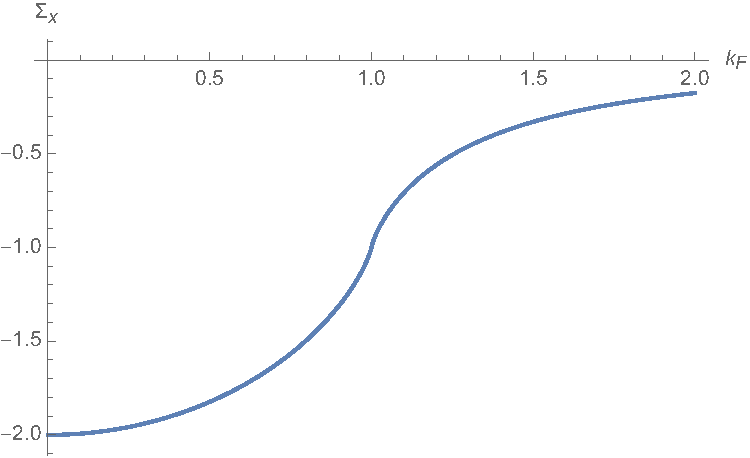
\includegraphics[width=0.4\linewidth]{./fig/fig5_1.pdf}
    \caption{Exchange energy.}%
    \label{fig:5.1}
\end{figure}
The behaviour of the function is in shown in Figure~\ref{fig:5.1}.

The derivative has a logarithmic divergence as $y\to 1$. This fact is interesting because it predicts that the effective mass is zero.
The effective mass of a particle defined in \eqref{3.160}.
Since the exchange self-energy is not frequency dependent, the effective mass is
\begin{equation}
    \left( \frac{m}{m^*} \right) = 1+ \partial_{\varepsilon_k} \Sigma_x(k) = \frac{e^2 m}{2\pi k_F } \frac{1}{y^2} \left( \frac{1+y^2}{y} \ln \abs{ \frac{1+y}{1-y} }-1  \right) \label{5.24}
\end{equation}
which diverges at Fermi energy $y\to 1$.
If the inverse effective mass really diverged at the Fermi surface, it would have several observable consequences.
The electron gas would be unstable at low temperatures, and the specific heat would diverge.
Further terms in the perturbation theory produces another divergence in the effective mass which exactly cancels the one due to exchange.
The effective mass and specific heat are not divergent.

The exchange energy contribution to the ground state energy is obtained from \eqref{5.12}.
Summing over spin gives an expression
\begin{eqnarray}
    E_{gx} &=& \frac{1}{N_e} \sum_\bk n_\bk \Sigma_x(k) = \frac{1}{n_0} \int \frac{d^3k}{(2\pi)^3} n_k \Sigma_x(k) \nonumber \\
    &=& - \frac{3}{4} \frac{e^2 k_F}{\pi} \label{5.25}
\end{eqnarray}
The average exchange energy per electron is $ \frac{3}{2} $ of the value ate the Fermi energy.
In therms of the parameter $r_s$, the total ground state exchange energy per electron is
\begin{equation}
    E_{gx} = - \frac{3}{2\pi} (k_F a_0) \left( \frac{e^2}{2a_0} \right) = - \frac{0.9163}{r_s} \label{5.26}
\end{equation}

So far two terms have been found for the energy of the particle,
\begin{equation}
    E(k) = \frac{\hbar^2 k^2}{2m} + \Sigma_x(k) + \dots \label{5.27}
\end{equation}
The corresponding two terms for the ground state energy per particle are,
\begin{equation}
    E_g = \frac{2.2099}{r_s^2} - \frac{0.9163}{r_s} + \dots \label{5.28}
\end{equation}
The ground state energy has the appearance of a power series, in increasing powers of $r_s$.
Although it is usually unsafe to extrapolate from just two terms, in fact $E_g$ is a series in $r_s$.
The next term will be of order $O(r_s^0)$.
The zeroth power could be interpreted as either a constant or as $\ln(r_s)$.
The series have the form
\begin{equation}
    E_g =  \frac{2.2099}{r_s^2} - \frac{0.9163}{r_s} -0.094 + 0.0622\ln(r_s) + \dots \label{5.29}
\end{equation}

The above energy terms comprise the Hartree-Fock theory.
It is defined to be the kinetic energy, the Hartree energy which is zero, and the exchange energy.
The total ground state energy per particle is written with correlation energy,
\begin{equation}
    E_g = \frac{2.2099}{r_s^2} - \frac{0.9163}{r_s} +E_c \label{5.30}
\end{equation}
where the correlation energy $E_c$ needs to be determined.
The result
\begin{equation}
    E_c = -0.094 + 0.0622\ln(r_s) + O(r_s) \label{5.31}
\end{equation}
is convergence when $r_s \leq 1$.

\subsection{Seitz's Theorem}
The theorem of Seitz relates the ground state energy to the chemical potential.
The chemical potential is defined as the energy it takes to add or remove an electron from the material.
It is the energy which divides the empty from the occupied states at zero temperature.
Of course, it is just the Fermi energy of the metal.
The chemical potential is the energy of an electron of momentum $k_F$
\begin{equation}
    \mu = \frac{\hbar^2 k_F^2}{2m} + \Sigma_x (k_F) + \Re \Sigma_c(k_f,0) \label{5.33}
\end{equation}
where $ik_n= 0$ is the chemical potential.
The chemical potential $\mu$ is only a function of the electron $n_0$. The theorem of Seitz is
\begin{equation}
    \mu (n_0)  = \frac{d}{d n_0}  \left[ n_0 E_g(n_0) \right] = E_g + n_0 \frac{d E_g}{d n_0} \label{5.34}
\end{equation}
The proof, by definition of chemical potential
\begin{equation}
    \mu = E_T(N_e+1) - E_T(N_e)     \label{5.35}
\end{equation}
The total energy for $N_e$ particle system is $E_T = N_e E_g$ for a fixed volume since the $E_g$ is the function of density,
\begin{eqnarray}
    E_T(N_e+1) &=& (N_e+1) E_g(n_0 + 1/V) = (N_e+1) \left( E_g(n_0) + \frac{1}{V} \frac{d E_g}{d n_0} \right) \nonumber \\
    &=& N_e E_g + E_g(n_0) + n_0 \frac{dE_g}{n_0}  + O( \frac{1}{V} )   \label{5.36}
\end{eqnarray}
In proving the theorem, the volume $V$ is kept fixed, as is the amount of positive charge.
The $N_e+1$ particle system has a slight charge imbalance, but it is negligible to the contribution of energy.
Considering a body of average dimension $L$ is uniformly charged with on unit of charge, the Coulomb energy is of order $e^2/L$.
This contribution is negligible when $L$ is large.

The chemical potential is the negative of the work function.
It is the energy required to remove an electron form the solid and take it to infinity with zero kinetic energy.
However, there is a surface correction to the work function, but not to volume part of the ground state energy per particle.
\begin{equation}
    E_T = N_e E_g + A E_S   \label{5.37}
\end{equation}
where $A$ is the total surface area and $E_S$ is the energy per unit surface area.
For macroscopic bodies, $E_g$ does not depend on the surface area.
However, $\mu$ does have a term which depends on the surface--actually on the surface dipole layer, $\mu = \mu_B + \Delta \mu$.
The theorem of Seitz actually just works on $\mu_B$.
In Hartree-Fock approximation the chemical potential gives for the bulk contribution,
\begin{equation}
    \mu_{B,HF} = \frac{d}{dn_0} \left( n_0 E_{g,HF} \right) = E_F - \frac{e^2 k_F}{\pi}     \label{5.39}
\end{equation}

\subsection{$\Sigma^{2a}$}
The exchange energy calculated involve one Coulomb line.
The correlation energy is the sum of all contribution with two or more Coulomb lines.
There are three diagrams with two Coulomb line.
\begin{figure}[ht]
    \centering
    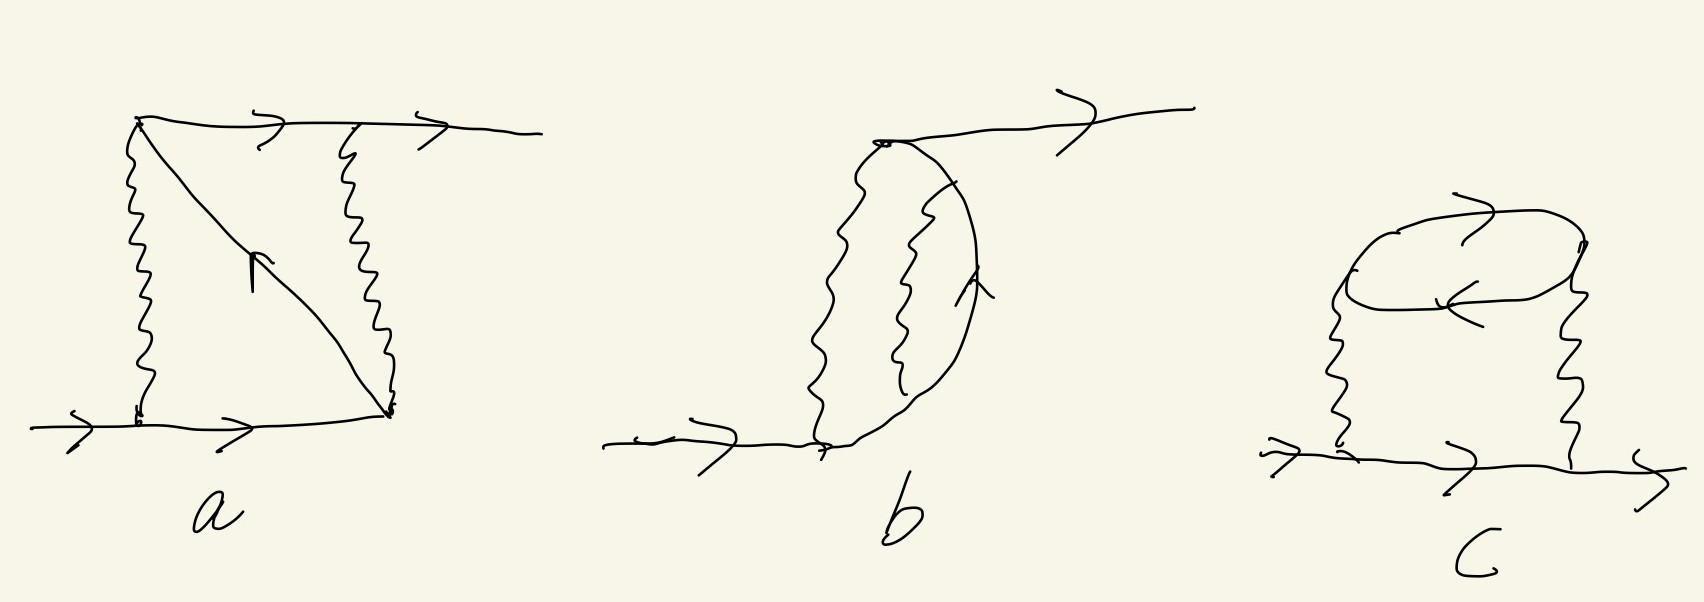
\includegraphics[width=0.8\linewidth]{./fig/fig5-2.jpg}
    \caption{Diagrame}%
    \label{fig:5.2}
\end{figure}

For Figure~\ref{fig:5.2}a, the self-energy contribution is
\begin{equation}
    \Sigma^{2a}(k) = \frac{1}{V^2\beta^2} \sum_{\bq \bq'} v_q v_{q'} \sum_{iq_n,iq_{ n'}} \cg^0(k+q) \cg^0(k+q') \cg^0(k+q+q')
\end{equation}
according \eqref{3.217} and calculation, we have
\begin{eqnarray}
    \Sigma^{2a}(k) &=& - \frac{1}{V^2} \sum_{\bq \bq'} \frac{v_q v_{q'}}{ik_n + \xi_{\bk+\bq+\bq'} - \xi_{\bk+\bq'} -\xi_{\bk+\bq} } \nonumber \\
    &=& \left[ \eta_F(\xi_{\bk+\bq'}) \left( \eta_F(\xi_{\bk+\bq}) - \eta_F(\xi_{\bk+\bq+\bq'})  \right) \right. \nonumber\\
    &+&\left. \eta_F(\xi_{\bk+\bq+\bq'})\left( 1- \eta_F(\xi_{\bk+\bq} \right) \right]
\end{eqnarray}
The self-energy of a particle is needed on the Fermi surface.
Set $k=k_F$ and $ik_n = \xi_{k_F} =k_F^2/2m - \mu = 0$.
The terms in the energy denominator largely cancel,
\begin{equation}
    \xi_\bk + \xi_{\bk+\bq+\bq'} - \xi_{\bk+\bq} - \xi_{\bk+ \bq'} = \frac{\bq \cdot \bq'}{m}   \label{5.44}
\end{equation}
The self-energy is
\begin{eqnarray}
    \Sigma^{2a}(k_F,0) &=& - \frac{(4\pi e^2)^2 m}{(2\pi)^6} \int \frac{d^3 q}{q^2} \int \frac{d^3 q'}{(q')^2} \frac{1}{\bq \cdot \bq'} \nonumber \\
    &\times& \{ \eta_F(\xi_{\bk+\bq'}) \left[ \eta_F(\xi_{\bk+\bq}) - \eta_F(\xi_{\bk+\bq+\bq'})  \right] + \dots  \} \label{5.45}
\end{eqnarray}
The quantity on the right is independent of the electron density.
The integral is convergent and give nonzero result.
It contribute the constant term in $E_c$.
With further calculation by Onsager, we have
\begin{equation}
    \Sigma^{2a} = \frac{1}{3} \ln(2) - \frac{3}{2\pi^2}  \zeta(3) = 0.0436
\end{equation}

\subsection{$\Sigma^{2b}$}
The second self-energy term involving two Coulomb lines is shown in Figure~\ref{fig:5.2}b, this contribution can be shown equal to zero.
Consider the summation of the similar diagrams, all terms may be summed by evaluating the exchange energy with an electron Green's function in the self-energy which includes the exchange energy.
This summation is given by the self-energy
\begin{equation}
    \Sigma'_x(k) = - \frac{1}{V\beta} \sum_{\bq,ik_n} v_q \cg(\bk+\bq,ik_n) \label{5.47}
\end{equation}
\begin{equation}
    \cg (\bk+\bq,ik_n) = \frac{1}{ik_n - \xi_{\bk+\bq} -\Sigma_x(\bk+\bq)} \label{5.48}
\end{equation}
where the Green's function has a self-energy due to exchange.
